\chapter{Diferenciación e Integración numérica}

La diferenciación, y sobre todo la integración son operaciones habituales en cálculo numérico. En muchos casos obtener la expresión analítica de la derivada o la integral de una función puede ser muy complicado o incluso imposible. Además en ocasiones no disponemos de una expresión analítica para la función que necesitamos integrar o derivar, sino tan solo de un conjunto de valores numéricos de la misma. Este es el caso, por ejemplo, cuando estamos trabajando con datos experimentales. Si solo disponemos de valores numéricos, entonces solo podemos calcular la integral o la derivada numéricamente.

Los sistemas físicos se describen generalmente mediante ecuaciones diferenciales.  La mayoría de las ecuaciones diferenciales no poseen una solución analítica, siendo posible únicamente obtener soluciones numéricas. 

En términos generales la diferenciación numérica consiste en aproximar el valor que toma la derivada de una función en un punto. De modo análogo, la integración numérica aproxima el valor que toma la integral de una función en un intervalo.

\section{Diferenciación numérica.}

Como punto de partida, supondremos que tenemos un conjunto de puntos $\{x_i,y_i\}$,
\begin{table}[h]
\centering
\begin{tabular}{c|cccc}
x&$x_0$&$x_1$&$\cdots$&$x_n$\\
\hline
y&$y_0$&$y_1$&$\cdots$&$y_n$
\end{tabular}
\end{table} 

Que pertenecen a una función $y=f(x)$ que podemos o no conocer analíticamente. El objetivo de la diferenciación numérica es estimar el valor de la derivada $f'(x)$ de la función, en alguno de los puntos $x_i$ en los que el valor de $f(x)$ es conocido. 

En general existen dos formas de aproximar la derivada:

\begin{enumerate}
\item Derivando el polinomio de interpolación. De este modo, obtenemos un nuevo polinomio que aproxima la derivada.
\begin{equation*}
f(x)\approx P_n(x) \Rightarrow f'(x) \approx P'_n(x)
\end{equation*}

\item Estimando la derivada como una fórmula de diferencias finitas obtenida a partir de la aproximación del polinomio de Taylor. 

Si partimos de la definición de derivada, 
\begin{equation*}
f'(x_0)=\lim_{h\rightarrow 0}\frac{f(x_0+h)-f(x_0)}{h} \approx \frac{f(x_0+h)-f(x_0)}{h} 
\end{equation*}
\end{enumerate}

Podemos asociar esta aproximación con el polinomio de Taylor de primer orden de la función $f(x)$,

\begin{equation*}
f(x)\approx f(x_0)+f'(x_0)\cdot(x-x_0) \Rightarrow f'(x_0)\approx \frac{f(x)-f(x_0)}{x-x_0}
\end{equation*}

Si hacemos $x-x_0=h$, ambas expresiones coinciden.
 
En general, los algoritmos de diferenciación numérica son inestables. Los errores iniciales que puedan contener los datos debido a factores experimentales o al redondeo del ordenador, aumentan en el proceso de diferenciación. Por eso no se pueden calcular derivadas de orden alto y, los resultados obtenidos de la diferenciación numérica deben tomarse siempre extremando la precaución.

\subsection{Diferenciación numérica basada en el polinomio de interpolación.}\index{Diferenciación! polinomio interpolador}

El método consiste en derivar el polinomio $P_n(x)$ de interpolación obtenido por alguno de los métodos estudiados en el capítulo \ref{interpolacion} y evaluar el polinomio derivada $P'_n(x)$ en el punto deseado.

Un ejemplo particularmente sencillo, para la expresión del polinomio derivada se obtiene  en el caso de datos equidistantes interpolados mediante el polinomio de Newton-Gregory,

\begin{equation*}
p_n(x)=y_0+\frac{x-x_0}{h}\Delta y_0+\frac{(x-x_1)\cdot (x-x_0)}{2\cdot h^2}\Delta^2 y_0+\cdots +\frac{(x-x_{n-1}) \cdots (x-x_1)\cdot (x-x_0)}{n! \cdot h^n}\Delta^n y_0
\end{equation*}

Si lo derivamos, obtenemos un nuevo polinomio,

\begin{align*}
p'_n(x)&=\frac{\Delta y_0}{h}+\frac{\Delta^2 y_0}{2\cdot h^2}\left[(x-x_1)+(x-x_0) \right] +\\
&+\frac{\Delta^3 y_0}{3! \cdot h^3}\left[(x-x_1)(x-x_2)+(x-x_0)(x-x_1)+(x-x_0)(x-x_2)\right]+\cdots +\\
&+\frac{\Delta^n y_0}{n! \cdot h^n}\sum_{k=0}^{n-1}\frac{(x-x_0)(x-x_1)\cdots (x-x_{n-1})}{x-x_k}
\end{align*}

Este polinomio es especialmente simple de evaluar en el punto $x_0$,

\begin{align*}
p'_n(x_0)&=\frac{\Delta y_0}{h}+\frac{\Delta^2 y_0}{2\cdot h^2}\overbrace{(x_0-x_1)}^{-h}+\cdots +
\frac{\Delta^n y_0}{n! \cdot h^n}[\overbrace{(x_0-x_1)}^{-h}\overbrace{(x_1-x_2)}^{-h}\cdots \overbrace{(x_n-x_{n-1})}^{-h}]\\
p'_n(x_0)&=\frac{1}{h}\left(\Delta y_0-\frac{\Delta^2 y_0}{2}+\frac{\Delta^3 y_0}{3}+\cdots +
\frac{\Delta^n y_0}{n}(-1)^{n-1}\right)
\end{align*}

Es interesante remarcar como en la expresión anterior, el valor de la derivada se va haciendo más preciso a medida que vamos añadiendo diferencias de orden superior. Si solo conociéramos dos datos, $(x_0, y_0)$ y $(x_1, y_1)$. Solo podríamos calcular la diferencia dividida de primer orden. En esta caso nuestro cálculo aproximado de la derivada de $x_0$ sería,
\begin{equation*}
p'_1(x_0)=\frac{1}{h}\Delta y_0
\end{equation*}

Si conocemos tres datos, podríamos calcular $\Delta^2y_0$ y añadir un segundo término a nuestra estima de la derivada,
\begin{equation*}
p'_2(x_0)=\frac{1}{h}\left(\Delta y_0-\frac{\Delta^2 y_0}{2}\right)
\end{equation*}

y así sucesivamente, mejorando cada vez más la precisión.

Veamos como ejemplo el cálculo la derivada en el punto $x_0=0.0$, a partir de la siguiente tabla de datos,

\begin{table}[h]
\centering
\begin{tabular}{cccccc}
$x_i$&$y_i$&$\Delta y_i$&$\Delta^2 y_i$&$\Delta^3 y_i$ & $\Delta^4 y_i$\\
\hline
$0.0$& $0.000$& $0.203$ &$0.017$ &$0.024$ &$0.020$\\
$0.2$ &$0.203$ &$0.220$ &$0.041$ &$0.044$\\
$0.4$ &$0.423$ &$0.261$ &$0.085$\\
$0.6$ &$0.684$ &$0.346$\\
$0.8$ &$1.030$\\
\end{tabular}
\end{table} 

\begin{itemize}
\item Empleando los dos primeros puntos,
\begin{equation*}
y'(0,0)=p_1^1(0.0)=\frac{1}{0.2}\cdot 0.203= 1.015
\end{equation*}
\item Empleando los tres primeros puntos,
\begin{equation*}
y'(0,0)=p_2^1(0.0)=\frac{1}{0.2}\left( 0.203-\frac{0.017}{2}\right)= 0.9725
\end{equation*}
\item Empleando los cuatro primeros puntos,
\begin{equation*}
y'(0,0)=p_3^1(0.0)=\frac{1}{0.2}\left( 0.203-\frac{0.017}{2}+\frac{0.024}{3}\right)= 1.0125
\end{equation*}
\item Empleando los cinco puntos disponibles
\begin{equation*}
y'(0,0)=p_4^1(0.0)=\frac{1}{0.2}\left( 0.203-\frac{0.017}{2}+\frac{0.024}{3}-\frac{0.020}{4}\right)= 0.9875
\end{equation*}
\end{itemize}

\subsection{Diferenciación numérica basada en diferencias finitas}
\index{Diferenciación! diferencias finitas}
Como se explicó en la introducción, la idea es emplear el desarrollo de Taylor para aproximar la derivada de una función en punto. Si empezamos con el ejemplo más sencillo, podemos aproximar la derivada suprimiendo de su definición el \emph{paso al límite}\index{Diferenciación!Diferencia adelantada de dos puntos},

\begin{equation*}
f'(x_k)=\lim_{h\rightarrow 0}\frac{f(x_k+h)-f(x_k)}{h} \approx \frac{f(x_k+h)-f(x_k)}{h} 
\end{equation*}

La expresión obtenida, se conoce con el nombre de formula de diferenciación adelantada de dos puntos. El error cometido debido a la elección de un valor de $h$ finito, se conoce con el nombre de error de truncamiento\index{Error de Truncamiento}. Es evidente que desde un punto de vista puramente matemático, la aproximación es mejor cuanto menor es $h$. Sin embargo, desde un punto de vista numérico esto no es así. A medida que hacemos más pequeño el valor de $h$, aumenta el error de redondeo debido a la aritmética finita del computador\index{Error de redondeo}. Por tanto, el error cometido es la suma de ambos errores,
\begin{equation*}
f'(x)=\frac{f(x+h)-f(x)}{h}+\overbrace{C\cdot h}^{\mathtt{e.\ de\  truncamiento}}+\underbrace{D\cdot \frac{1}{h}}_{\mathtt{e.\ de\  redondeo}}, \ C>>D 
\end{equation*}

El valor óptimo de $h$ es aquel que hace mínima la suma del error de redondeo y el error de truncamiento. La figura \ref{fig:errores} muestra de modo esquemático como domina un error u otro según hacemos crecer o decrecer el valor de $h$ en torno a su valor óptimo.

\begin{figure}[h]
\centering
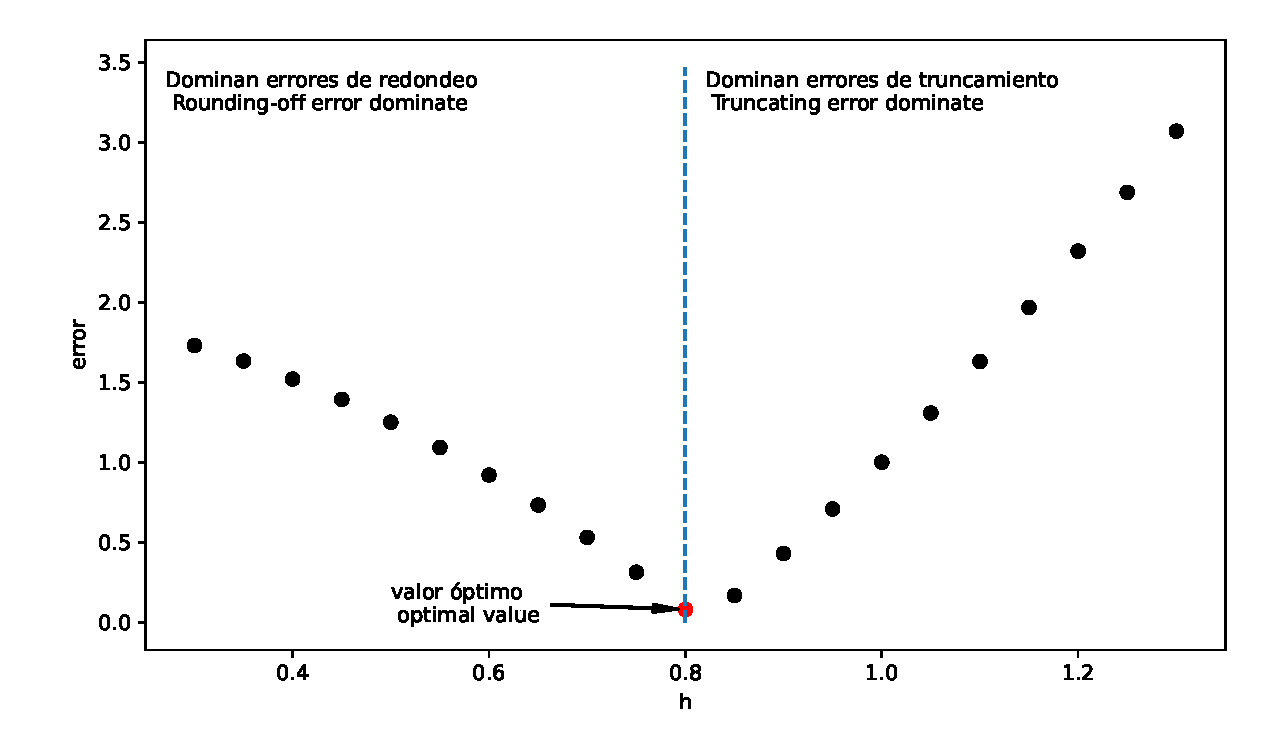
\includegraphics[width=12cm]{errores.eps}
\caption{Variación del error cometido al aproximar la derivada de una función empleando una fórmula de diferenciación de dos puntos.} 
\label{fig:errores}
\end{figure}

Como vimos en la introducción a esta sección, partiendo de el desarrollo de Taylor de una función es posible obtener fórmulas de diferenciación numérica y poder estimar el error cometido. Así por ejemplo, a  partir del polinomio de Taylor de primer orden,
\begin{equation*}
f(x+h)=f(x)+hf'(x)+\frac{h^2}{2}f''(z) \Rightarrow f'(x)=\frac{f(x+h)-f(x)}{h}-\frac{h}{2}f''(z), \ x<z<x+h
\end{equation*}

El error que se comete debido a la aproximación, es proporcional al tamaño del intervalo empleado $h$ La constante de proporcionalidad depende de la derivada segunda de la función, $f''(z)$ en algún punto indeterminado ($z\in x,x+h$). Para indicar esta relación lineal entre el error cometido y el valor de $h$, se dice que el error es del \emph{orden} de $h$ y se representa como $O(h)$.
\begin{equation*}
f'(x)=\frac{f(x+h)-f(x)}{h}+O(h)
\end{equation*}

\begin{figure}[h]
\centering
\subfigure[Diferencia de dos puntos adelantada \label{fig:diffin1}]{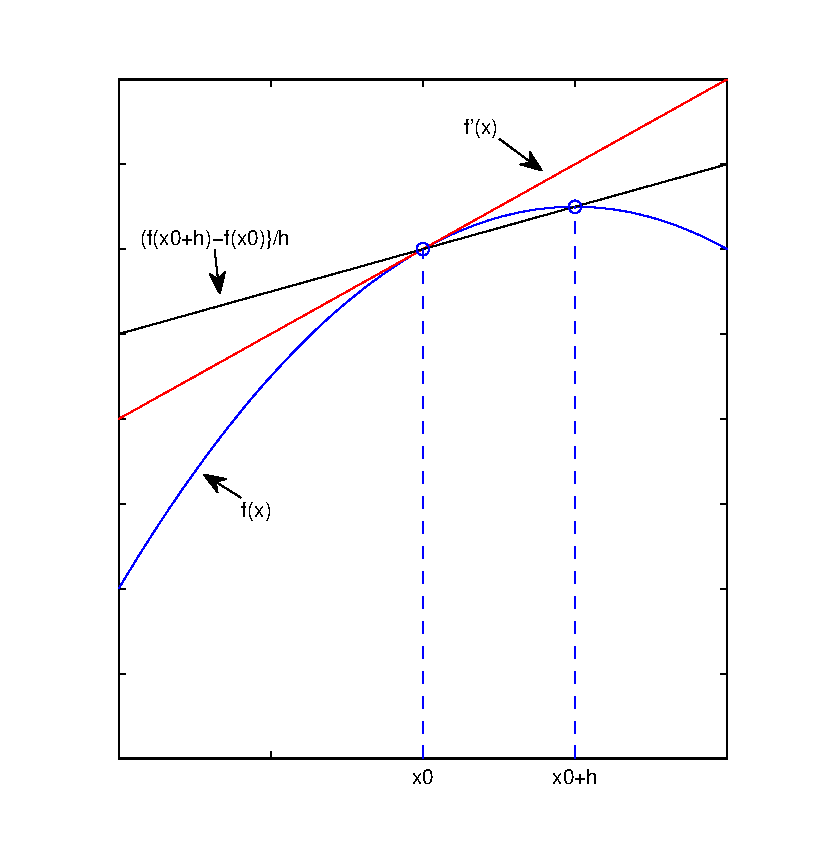
\includegraphics[width=7cm]{diffin1.eps}} \qquad 
\subfigure[Diferencia de dos puntos centrada \label{fig:diffin2}]{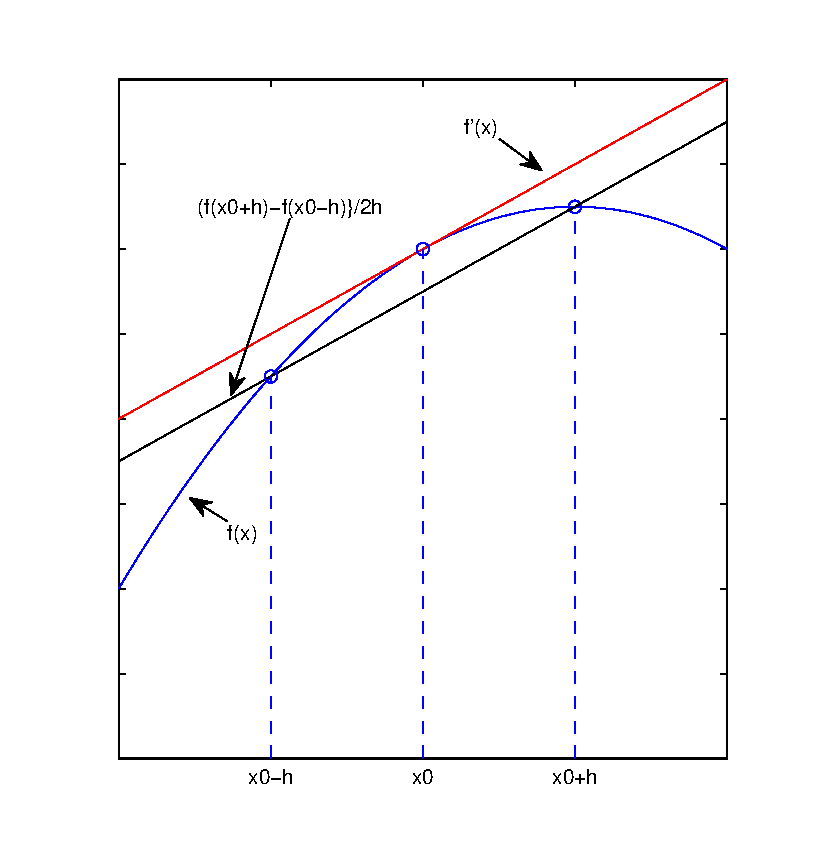
\includegraphics[width=7cm]{diffin2.eps}}
\caption{Comparación entre las aproximaciones a la derivada de una función obgtenidas mediante las diferencias de dos puntos adelantada y centrada} 
\label{fig:diffin}
\end{figure}

Podemos mejorar la aproximación, calculando el valor de polinomio de Taylor de tercer orden para dos puntos equidistantes situados a la izquierda y la derecha del punto x, restando dichas expresiones y despejando la derivada primera del resultado,

\begin{equation*}
\left. \begin{aligned}
f(x+h)=f(x)+hf'(x)+\frac{h^2}{2}f''(x)+\frac{h^3}{3!}f'''(z)\\
f(x-h)=f(x)-hf'(x)+\frac{h^2}{2}f''(x)-\frac{h^3}{3!}f'''(z)
\end{aligned} \right\rbrace \Rightarrow f'(x)=\frac{f(x+h)-f(x-h)}{2h}-\frac{h^2}{6}f'''(z) 
\end{equation*}

En esta caso, el error es proporcional al cuadrado de $h$, por tanto,

\begin{equation*}
f'(x_0)=\frac{f(x_1)-f(x_{-1})}
{2h}+O(h^2)
\end{equation*}

Donde hemos hecho $x\equiv x_0$, $x+h\equiv x_1$ y $x-h\equiv x_{-1}$. Esta aproximación recibe el nombre de diferencia de dos puntos centrada.\index{Diferenciación! Diferencia de dos puntos centrada} La figura \ref{fig:diffin1} muestra una comparación entre la derivada real de una función y su aproximación mediante una diferencia adelantada de dos puntos. La figura \ref{fig:diffin2} muestra la misma comparación empleando esta vez la aproximación de dos punto centrada. En este ejemplo es fácil ver como la aproximación centrada da un mejor resultado. No hay que olvidar que  la bondad del resultado, para un valor de $h$ dado, depende también del valor de las derivadas de orden superior de la función, por lo que no es posible asegurar que el resultado de la diferencia centrada sea siempre mejor.

Empleando el desarrollo de Taylor y tres puntos podemos aproximar la derivada por la diferencia de tres puntos adelantada,

\begin{align*}
\left. \begin{aligned}
4\cdot\left(f(x_1)=f(x_0)+hf'(x_0)+\frac{h^2}{2}f''(x_0)+\frac{h^3}{3!}f'''(z)\right)\\
f(x_2)=f(x_0)+2hf'(x_0)+2{h^2}{2}f''(x_0)+\frac{4h^3}{3}f'''(z)
\end{aligned} \right\rbrace \Rightarrow \\
\Rightarrow f'(x_0)=\frac{-f(x_2)+4f(x_1)-3f(x_0)}{2h}-\frac{h^2}{3}f'''(z) 
\end{align*} 

En este caso e error es también de  orden $h^2$ pero vale el doble que para la diferencia de dos puntos centrada.

A partir del desarrollo de Taylor y mediante el uso del número de puntos adecuado, es posible obtener aproximaciones a la derivada primera y a las sucesivas derivadas de una función, procediendo de modo análogo a como acaba de mostrarse para el caso de las diferencias de dos y tres puntos. La tabla \ref{tabdiff} muestra algunas de las fórmulas de derivación mediante diferencias finitas más empleadas. Para simplificar la notación, en todos los casos se ha tomado $y_i=f(x_i), \ y_i^{(j)}=f^{(j)}(x_i)$.

\begin{table}[h]
\centering
\begin{tabular}{|c|c|}
\hline
Fórmulas primera derivada & Fórmulas segunda derivada\\
\hline
\ & \\
$y'_0=\frac{y_1-y_0}{h}+O(h)$ & $y''_0=\frac{y_2-2y_1+y_0}{h^2}+O(h)$\\
\ & \\
$y'_0=\frac{y_1-y_{-1}}{2h}+O(h^2)$ &$y''_0=\frac{y_1-2y_0+y_{-1}}{h^2}$\\
\ & \\
$y'_0=\frac{-y_2+4y_1-3y_0}{2h}+O(h^2)$ &$y''_0=\frac{-y_3+y_2-5y_1+2y_0}{h^2}+O(h^2)$\\
\ & \\
$y'_0=\frac{-y_2+8y_1-8y_{-1}+y_{-2}}{12h}+O(h^4)$ &$y''_0=\frac{-y_2+16y_1-30y_0+16y_{-1}-y_{-2}}{12h^2}+O(h^4)$\\
\ & \\
\hline
Fórmulas tercera derivada & Fórmulas cuarta derivada\\
\hline
\ & \\
$y'''_0=\frac{y_3-3y_2+3y_1-y_0}{h^3}+O(h)$ &$y^{iv}_0=\frac{y_4-4y_3+6y_2-4y_1+y_0}{h^4}+O(h)$\\
\ & \\
$y'''_0=\frac{y_2-2y_1+2yx_{-1}-y_{-2}}{2h^3}+O(h^2)$ &$y^{iv}_0=\frac{y_2-4y_1+6y_0-4y_{-1}+y_{-2}}{h^4}+O(h^2)$\\
\ &  \\
\hline
\end{tabular}
\caption{Fórmulas de derivación basadas en diferencias finitas}
\label{tabdiff}
\end{table}


\section{Integración numérica.}

Dada una función arbitraria $f(x)$ es en muchos casos posible obtener de modo analítico su primitiva $F(x)$ de modo que $f(x)=F'(x)$. En estos casos, la integral definida de $f(x)$ en un intervalo $[a,b]$ puede obtenerse directamente a partir de su primitiva,
\begin{equation*}
I(f)=\int_a^bf(x)dx=F(x)\vert_a^b=F(b)-F(a)
\end{equation*}
Hay sin embargo muchos casos en los cuales se desconoce la función $F(x)$ y otros en los que ni siquiera se conoce la expresión de la función $f(x)$, como por ejemplo, cuando solo se dispone de una tabla de valores $\left\lbrace x_i,y_i=f(x_i) \right\rbrace$ para representar la función. En estos casos se puede aproximar la integral definida de la función $f(x)$ en un intervalo $[a,b]$, a partir de los puntos disponibles, mediante lo que se conoce con el nombre de una fórmula de cuadratura,

\begin{equation*}
I(f)=\int_a^bf(x)dx \approx \sum_{i=0}^nA_if(x_i)
\end{equation*}

Una técnica habitual de obtener los coeficientes $A_i$, es hacerlo de modo implícito a partir de la integración  de los polinomios de interpolación,

 \begin{equation*}
I(f)=\int_a^bf(x)dx \approx \int_a^bP_n(x)dx
\end{equation*}

Para ello, se identifican los extremos del intervalo de integración con el primer y el último de los datos disponibles, $[a,b]\equiv [x_0,x_n]$.

Así por ejemplo, a partir de los polinomios de Lagrange, definidos en la sección \ref{sec:lagranje},

\begin{equation*}
p(x)=\sum_{j=0}^n l_j(x)\cdot y_j
\end{equation*}

Podemos obtener los coeficientes $A_i$ como,

\begin{equation*}
I(f)=\int_a^bf(x)dx \approx \int_a^bP_n(x)dx=\int_{x_0}^{x_n}\left( \sum_{j=0}^n l_j(x)\cdot y_j \right) dx \Rightarrow A_j=\int_{x_0}^{x_n}l_j(x)dx
\end{equation*}

La familia de métodos de integración, conocidas como fórmulas de Newton-Cotes, puede obtenerse a partir del polinomio de interpolación de Newton-Gregory descrito en la sección \ref{sec:newgre}\index{Integración! Formulas de Newton-Cotes}. Supongamos que tenemos la función a integrar definida a partir de un conjunto de puntos equiespaciados a lo largo del intervalo de integración $\{(x_i,y_i)\}_{0,\cdots n}$. Podemos aproximar la integral $I(y)$ como,

\begin{equation*}
\int_{x_0}^{x_n}ydx \approx \int_{x_0}^{x_n}\left(y_0+\frac{x-x_0}{h}\Delta y_0+\frac{(x-x_0)(x-x_1)}{2!h^2}\Delta ^2 y_0+\cdots +\frac{(x-x_0)\cdots(x-x_{n-1})}{n!h^n}\Delta^n y_0 \right)
\end{equation*}

Las fórmulas de Newton-Cotes se asocian con el grado del polinomio de interpolación empleado en su obtención:

\begin{itemize}
\item Para $n=1$, se obtiene la regla del trapecio,
\begin{equation*}
I(y)=\int_{x_0}^{x_1}ydx \approx \frac{h}{2}(y_0+y_1)
\end{equation*}
\item Para $n=2$, se obtiene la regla de Simpson 
\begin{equation*}
I(y)=\int_{x_0}^{x_2}ydx \approx \frac{h}{3}(y_0+4y_1+y_2)
\end{equation*}
\item Para $n=3$, se obtiene la regla de 3/8 de Simpson
\begin{equation*}
I(y)=\int_{x_0}^{x_3}ydx \approx \frac{3h}{8}(y_0+3y_1+3y_2+y_3)
\end{equation*}
\end{itemize}

No se suelen emplear polinomios de interpolación de mayor grado debido a los errores de redondeo y a las oscilaciones locales que dichos polinomios presentan.
 
\subsection{La fórmula del trapecio.}

La fórmula del trapecio emplea tan solo dos puntos para obtener la integral de la función en el intervalo definido por ellos. \index{Integración! Fórmula del trapecio}

\begin{equation*}
I(y)=\int_{x_0}^{x_1}ydx \approx \int_{x_0}^{x_1}\left(y_0+\frac{x-x_0}{h}\Delta y_0\right)dx =y_0x+\left. \frac{\Delta y_0}{h}\frac{(x-x_0)^2}{2} \right\rvert_{x_0}^{x_1}=\frac{h}{2}(y_0+y_1)
\end{equation*}

La figura \ref{fig:trapecio} muestra gráficamente el resultado de aproximar la integral definida de una función $y=f(x)$ mediante la fórmula del trapecio. Gráficamente la integral coincide con el área del \emph{trapecio} formado por los puntos $(x_0,0)$, $(x_0,y_0)$, $(x_1,y_1)$ y $(x_1,0)$.  De ahí su nombre y la expresión matemática obtenida,

\begin{equation*}
I(y)=\frac{h}{2}(y_0+y_1)
\end{equation*}

que coincide con el área del trapecio mostrado en la figura.
\begin{figure}[h]
\centering
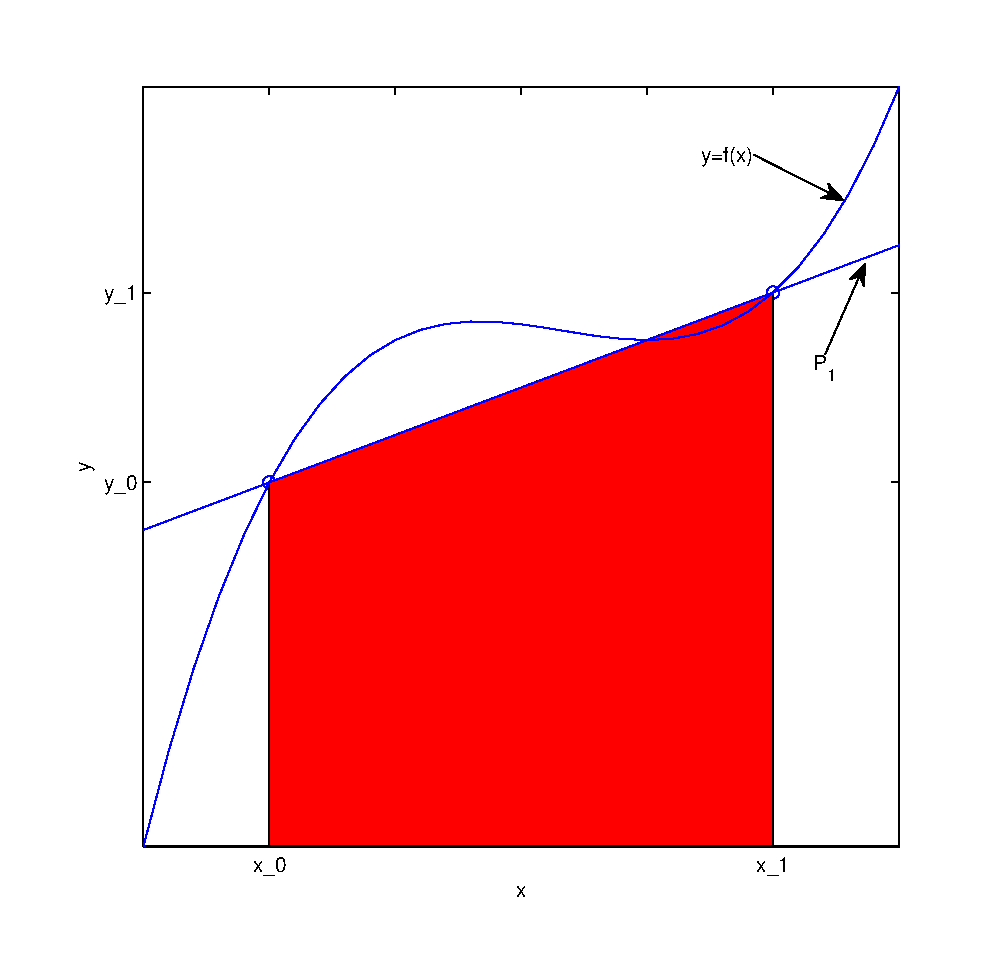
\includegraphics[width=9cm]{trapecio.eps}
\caption{Interpretación gráfica de la fórmula del trapecio.} 
\label{fig:trapecio}
\end{figure}

\paragraph*{Formula extendida (o compuesta) del trapecio.}\index{Integración! Fórmula compuesta del trapecio} La figura \ref{fig:trapecio} permite observar la diferencia entre el área calculada y el área comprendida entre la curva real y el eje $x$. Como se ha aproximado  la curva en el intervalo de integración por un línea recta (polinomio de grado 1 $p_1$), El error será tanto mayor cuando mayor sea el intervalo de integración y/o la variación de la función en dicho intervalo. Una solución a este problema, si se conoce la expresión analítica de la función que  se desea integrar o se conocen suficientes puntos es subdividir el intervalo de integración en intervalos más pequeños y aplicar a cada uno de ellos la fórmula de trapecio,

\begin{equation*}
I(y)=\int_{x_0}^{x_n}ydx \approx \sum_{i=0}^{n-1}\int_{x_i}^{x_{i+1}}y(x)dx=\sum_{i=0}^{n-1}\frac{h}{2}(y_i+y_{i+1})=\frac{h}{2}\left(y_0+2y_1+2y_2+\cdots+2y_{n-1}+y_n \right)
\end{equation*}

La figura \ref{fig:trapecio2}, muestra el resultado de aplicar la fórmula extendida del trapecio a la misma función de la figura \ref{fig:trapecio}. En este caso, se ha dividido el intervalo de integración en cuatro subintervalos. Es inmediato observar a partir de la figura, que la aproximación mejorar progresivamente si se aumenta el número de subintervalos y se reduce el tamaño de los mismos.

\begin{figure}[h]
\centering
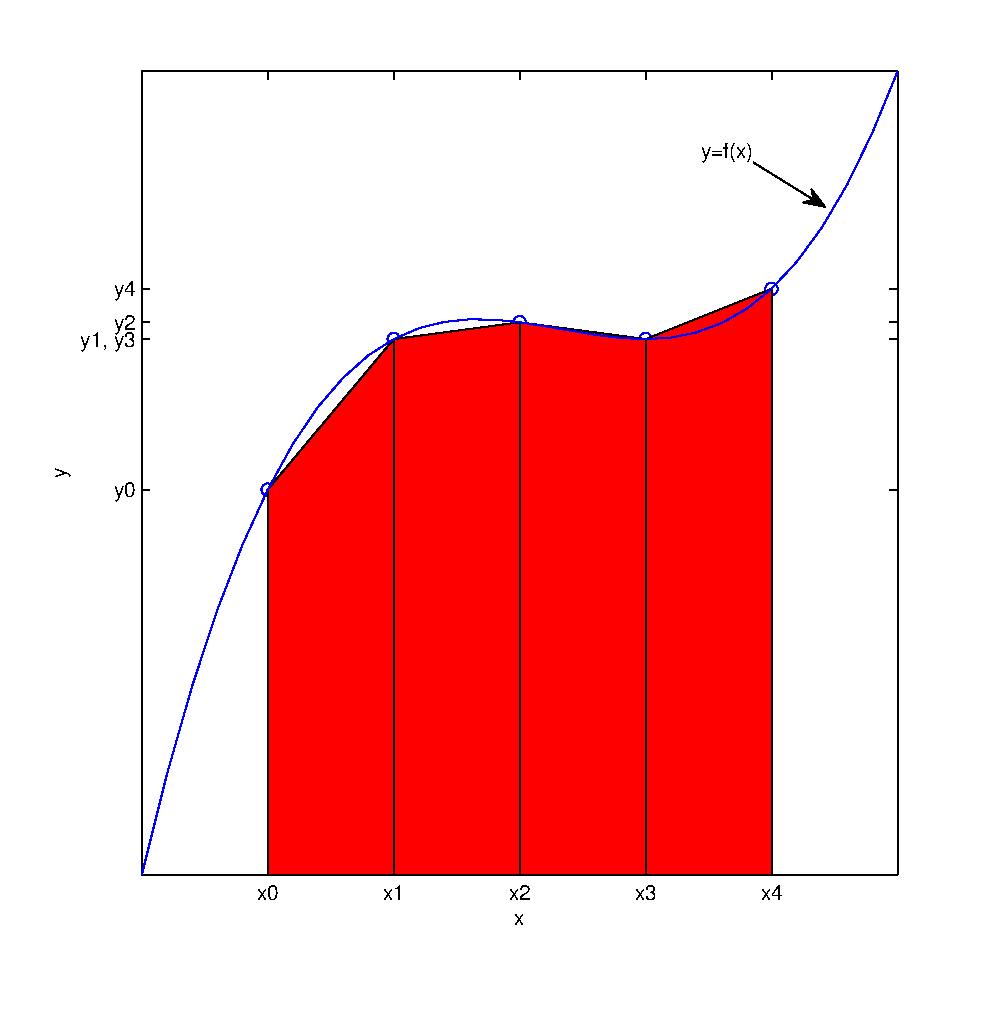
\includegraphics[width=9cm]{trapecio2.eps}
\caption{Interpretación gráfica de la fórmula extendida del trapecio.} 
\label{fig:trapecio2}
\end{figure}

\section{Las fórmulas de Simpson.}
Se conocen con el nombre de fórmulas integrales de Simpson, a las aproximaciones a la integral definida obtenida a partir de los polinomios interpoladores de Newton-Gregory de grado dos (Simpsom $1/3$) y de grado tres (Simpsom $3/8$) . \index{Integración! Fórmulas de Simpson}

En el primer caso, es preciso conocer tres valores equiespaciados de la función en el intervalo de integración y en el segundo es preciso conocer cuatro puntos. 

\paragraph*{Fórmula de Simpsom $1/3$.} La fórmula de Simpson, o Simpsom $1/3$,  emplea un polinomio de interpolación de Newton-Gregory de grado dos para  obtener la aproximación a la integral,

\begin{equation*}
I(y)\approx \int_{x_0}^{x_2}P_2(x)dx=\int_{x_0}^{x_2}\left(y_0+\frac{x-x_0}{h}\Delta y_0+\frac{(x-x_0)\cdot(x-x_1)}{2h^2}\Delta^2 y_0 \right)dx= \frac{h}{3}(y_0+4y_1+y_2)
\end{equation*}

La figura \ref{fig:simpsom}, muestra gráficamente el resultado de aplicar el método de Simpsom a la misma función de los ejemplos anteriores.  De nuevo, la bondad de la aproximación depende de lo que varíe la función en el intervalo.  La diferencia fundamental con el método del trapecio es que ahora el área calculada esta limitada por el segmento de parábola definido por el polinomio de interpolación empleado.

\begin{figure}[h]
\centering
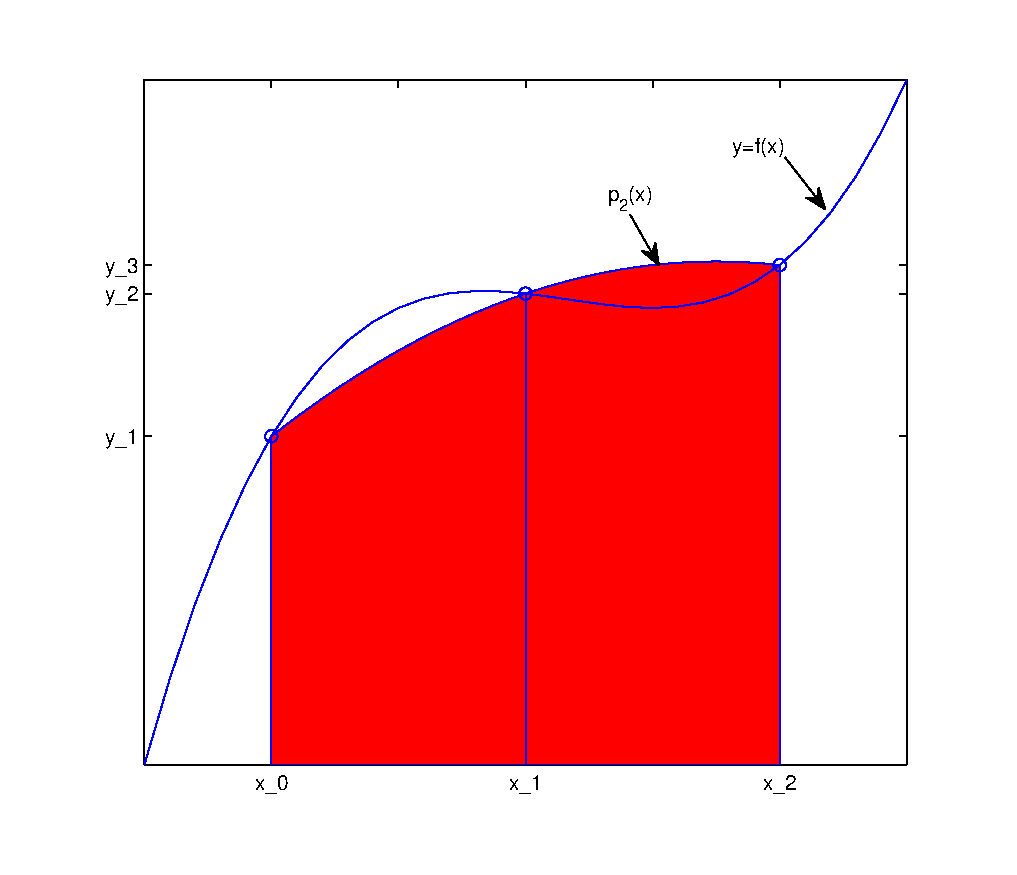
\includegraphics[width=8cm]{simpsom.eps}
\caption{Interpretación gráfica de la fórmula $1/3$ de Simpsom.} 
\label{fig:simpsom}
\end{figure}

\paragraph*{Fórmula de Simpsom $3/8$.} En este caso, se emplea un polinomio de Newton-Gregory de grado 3 para obtener la aproximación a la integral,

\begin{align*}
I(y)&\approx \int_{x_0}^{x_2}P_2(x)dx=\\
&=\int_{x_0}^{x_2}\left(y_0+\frac{x-x_0}{h}\Delta y_0+\frac{(x-x_0)\cdot(x-x_1)}{2h^2}\Delta^2 y_0 +\frac{(x-x_0)\cdot(x-x_1)\cdot (x-x_2)}{3!h^3}\Delta^3 y_0\right)dx\\
&= \frac{3h}{8}(y_0+3y_1+3y_2+y_3)
\end{align*}

La figura  \ref{fig:simpsom38} muestra el resultado de aplicar la fórmula de Simpsom $3/8$ a la misma función de los ejemplos anteriores. En este caso, la integral sería exacta porque la función de ejemplo elegida es un polinomio de tercer grado y coincide exactamente con el polinomio de interpolación construido para obtener la integral.

\begin{figure}[h]
\centering
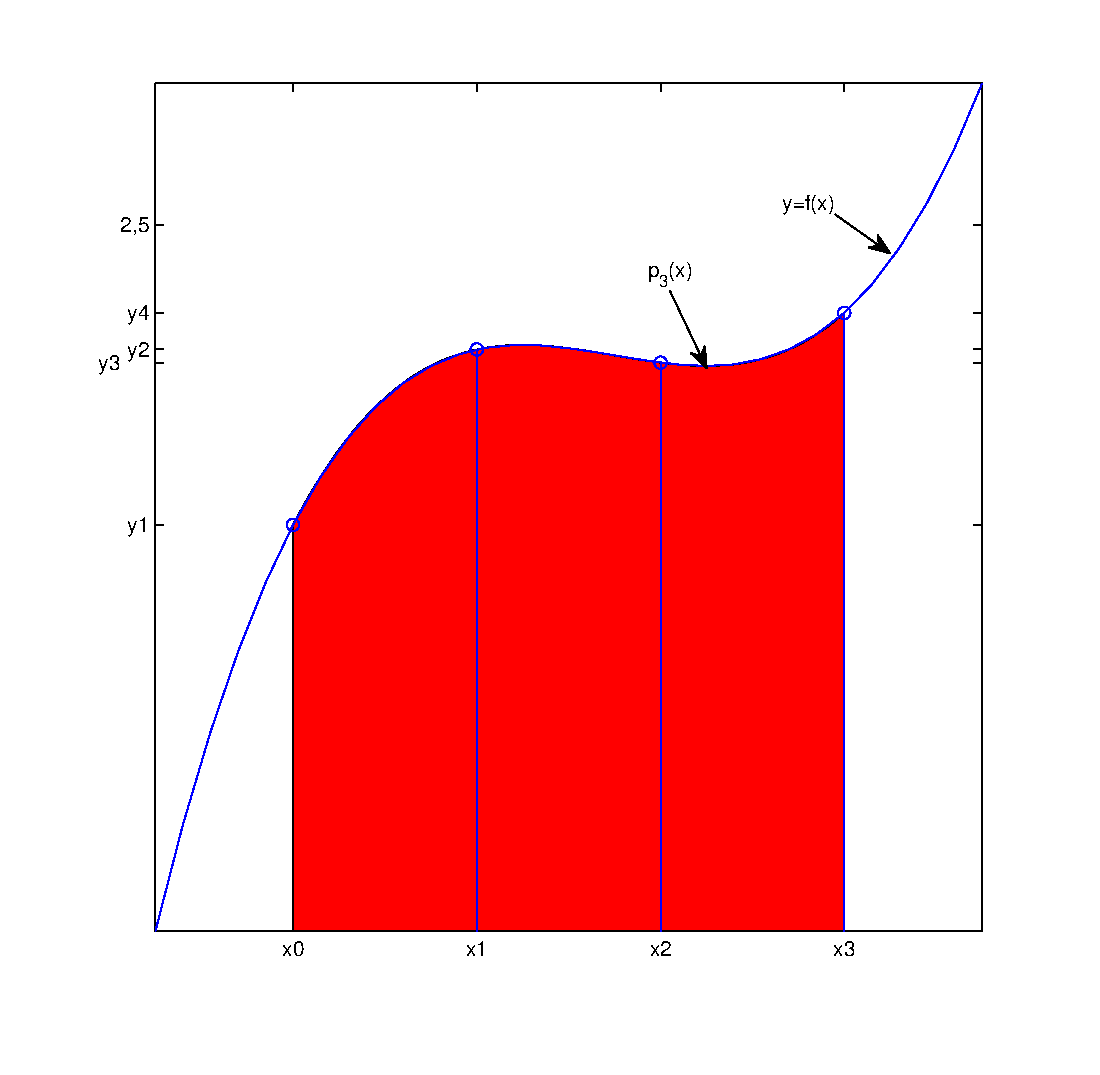
\includegraphics[width=9cm]{simpsom38.eps}
\caption{Interpretación gráfica de la fórmula $3/8$ de Simpsom.} 
\label{fig:simpsom38}
\end{figure}

Al igual que en el caso del método del trapecio, lo normal no es aplicar los métodos de Simpsom a todo el intervalo de integración, sino dividirlo en subintervalos más pequeños y aplicar el método sobre dichos subintervalos. El resultado se conoce como métodos extendidos de Simpsom. Al igual que sucede con la fórmula del trapecio, los métodos extendidos de Simpsom mejoran la aproximación obtenida para la integral tanto más cuanto más pequeño es el tamaño de los subintervalos empleados. 

Así, la fórmula extendida de Simpsom $1/3$ toma la forma,
 
\begin{align*}
I(y)&\approx \sum_{i=0}^{n-2}\int_{x_i}^{x_{i+2}}P_2(x)dx=\sum_{i=0}^{n-2}\frac{h}{3}(y_i+4y_{i+1}+y_{i+2})\\
&= \frac{h}{3}(y_0+4y_1+2y_2+4y_3+2y_4+\cdots + 2y_{n-2}+4y_{n-1}+y_n)
\end{align*}

Donde se ha dividido el intervalo de integración en $n$ subintervalos, la fórmula de Simpsom se ha calculado para cada dos subintevalos y se han sumado los resultados.

Por último para la fórmula extendida de Simpsom $3/8$ se puede emplear la expresión,

\begin{align*}
I(y)&\approx \sum_{i=0}^{n-2}\int_{x_i}^{x_{i+2}}P_3(x)dx=\sum_{i=0}^{n-2}\frac{3h}{8}(y_i+3y_{i+1}+3y_{i+2}+y_{i+3})\\
&= \frac{3h}{8}(y_0+3y_1+3y_2+2y_3+3y_4+3y_5+2y_6+ \cdots + 2y_{n-3}+3y_{n-2}+3y_{n-1}+y_n)
\end{align*}

En este caso también se divide el intervalo en $n$ subintervalos pero ahora se ha aplicado la regla de Simpsom $3/8$ a cada tres subintevalos.

A continuación se incluye un código que permite permite aproximar la integral definida de una función en un intervalo por cualquiera de los tres métodos descritos: Trapecio, Simpsom o Simpsom $3/8$,

\begin{verbatim}
function int=integra(fun,met,inter,dib)
%implementa los metodos del trapecio, etc...
%Uso: int=integra(fun,inter,dib)
%fun, nombre de la función que se desea intergrar, debe ir entre comillas
%met, método que se desea emplear para calcular la integral. los nombres
%validos para los metodos son: 'trapecio', 'simpson' y simpsom38'
%inter, es un vector de dos elementos que contiene lo extremos de intervalo
%de integracion [a,b]
%dib, si se da un valor a esta variable de entrada, dibuja la función en el
%intervalo de integración y la integral obtenida. Si se omite no dibuja
%nada.
%int, valor de la integral obtenida.
%Este programa no divide el intervalo de integración en subintervalos...
%para calcular la integral empleando subintervalos usar la función trocea,

if strcmp(met,'trapecio')
    f0=feval(fun,inter(1));
    f1=feval(fun,inter(2));
    h=inter(2)-inter(1);
    int=h*(f0+f1)/2;
    if nargin==4
        x=inter(1):(inter(2)-inter(1))/100:inter(2);
        yfuncion=feval(fun,x);
        ypolinomio=f0+(x-inter(1))*(f1-f0)/h;
        plot(x,yfuncion,x,ypolinomio,'r')
        hold on
        fill([x(1) x x(length(x))],[0 ypolinomio 0],'r') 
    end
elseif strcmp(met,'simpson')
    pmedio=(inter(2)+inter(1))/2;
    f0=feval(fun,inter(1));
    f1=feval(fun,pmedio);
    f2=feval(fun,inter(2));
    h=(inter(2)-inter(1))./2;
    int=h*(f0+4*f1+f2)/3;
    if nargin==4
        x=inter(1):(inter(2)-inter(1))/100:inter(2);
        yfuncion=feval(fun,x);
        ypolinomio=f0+(x-inter(1)).*(f1-f0)/h+(x-inter(1)).*(x-pmedio).*(f2...
        -2*f1+f0)./(2*h^2);
        plot(x,yfuncion,x,ypolinomio,'r')
        hold on
        fill([x(1) x x(length(x))],[0 ypolinomio 0],'r') 
    end        
elseif strcmp(met,'simpsom38')
    inter=inter(1):(inter(2)-inter(1))/3:inter(2);

    f=feval(fun,inter);
    h=(inter(4)-inter(1))/3;
    int=3*h*(f(1)+3*f(2)+3*f(3)+f(4))/8;
    if nargin==4
        x=inter(1):(inter(4)-inter(1))/100:inter(4);
        yfuncion=feval(fun,x);
        ypolinomio=f(1)+(x-inter(1)).*(f(2)-f(1))/h+(x-inter(1)).*(x...
        -inter(2)).*(f(3)-2*f(2)+f(1))./(2*h^2)+(x-inter(1)).*(x...
        -inter(2)).*(x-inter(3)).*(f(4)-3*f(3)+3*f(2)-f(1))./(6*h^3);
        plot(x,yfuncion,x,ypolinomio,'r')
        hold on
        fill([x(1) x x(length(x))],[0 ypolinomio 0],'r') 
    end
else
    int='metodo desconocido, los metodos conocidos son ''trapecio'', ...
    ''simpson' y ''simpsom38'''
end
\end{verbatim}

Este programa aplica directamente el método deseado sobre el intervalo de integración. Para obtener los métodos extendidos, podemos emplear un segundo programa que divida el intervalo de integración inicial en el número de subintervalos que deseemos, aplique el programa anterior a cada subintervalo, y, por último, sume todo los resultados para obtener el valor de la integral en el intervalo deseado. El siguiente programa, muestra un ejemplo de como hacerlo,

\begin{verbatim}
function total=trocea(fun,met,inter,div,dib)
%esta funcion lo unico que hace es trocear un intervalo en el numero de
%tramos indicados por div, y llamar a la funcion integra para que integre
%en cada intervalo.
%USO: total=trocea(fun,met,inter,div,dib)
% las variables de emtrada son la mismas que las de integra, salvo div que
% representa el numero de subintervalos en que se desea dividir el
% intervalo de integración.
tramos=inter(1):(inter(2)-inter(1))/div:inter(2);
total=0;
if nargin==5
    hold on
end
for i=1:size(tramos,2)-1
    int=integra(fun,met,[tramos(i) tramos(i+1)],dib);
    total=total+int;
end
hold off
\end{verbatim}t

Por último indicar que Matlab posee un comando propio para calcular la integral definida de una función, el comando \texttt{quad}. Este comando admite como variables de entrada el nombre de una función, y dos valores que representan los límites de integración. Como variable de salida devuelve el valor de la integral definida en el intervalo introducido. Por ejemplo,

\begin{verbatim}
>> i=quad('sin',0,pi)

i =

    2.0000
\end{verbatim}


\section{Problemas de valor inicial en ecuaciones diferenciales}
Las leyes de la física están escritas en forma de ecuaciones diferenciales. \index{Ecuación diferencial} \index{Problemas de valor inicial}

Una ecuación diferencial establece una relación matemática entre una variable y sus derivadas respecto a otra u otras variables de las que depende. El ejemplo más sencillo lo encontramos en las ecuaciones de la dinámica en una sola dimensión que relacionan la derivada segunda de la posición de un cuerpo con respecto al tiempo, con la fuerza que actúa sobre el mismo.

\begin{equation*}
m\cdot \frac{d^2x}{dt^2}=F
\end{equation*}

Si la fuerza es constante, o conocemos explícitamente como varía con el tiempo, podemos integrar la ecuación anterior para obtener la derivada primera de la posición con respecto al tiempo ---la velocidad--- de una forma directa,

\begin{equation*}
m\cdot \frac{d^2x}{dt^2}=F \rightarrow v(t)=\frac{dx}{dt}=\int \frac{F(t)}{m}dt +v(0)
\end{equation*}

Donde suponemos conocido el valor $v(0)$ de la velocidad del cuerpo en el instante inicial.

Si volvemos a integrar ahora la expresión obtenida para la velocidad, obtendríamos la posición en función del tiempo,

\begin{equation*}
v(t)=\frac{dx}{dt}=\int \frac{F(t)}{m}dt +v(0)\rightarrow x(tt)=\int\left(\int \frac{F(t)}{m}dt +v(0)\right)dt+x(0)
\end{equation*}

Donde suponemos conocida la posición inicial $x(0)$.

Quizá el sistema físico idealizado más conocido y estudiado es el oscilador armónico. En este caso, el sistema está sometido a una fuerza que depende de la posición y, si existe disipación, a una fuerza que depende de la velocidad,

\begin{equation*}
m\frac{d^2x}{dt}=-kx-\mu \frac{dx}{dt}+F(t)
\end{equation*}

En este caso, la expresión obtenida constituye una ecuación diferencial ordinaria y ya no es tan sencillo obtener una expresión analítica para x(t). Para obtener dicha expresión analítica, es preciso emplear métodos de resolución de ecuaciones diferenciales.

El problema del oscilador armónico, pertenece a una familia de problemas conocida como problemas de valores iniciales. En general, un problema de valores iniciales de primer orden consiste en obtener la función $x(t)$, que satisface la ecuación,
\begin{equation*}
x'(t)\equiv \frac{dx}{dt}=f(x(t),t), \ x(t_0)
\end{equation*}

Donde $x(t_0)$ representa un valor inicial conocido de la función $x(t)$.

En muchos casos, las ecuaciones diferenciales que describen los fenómenos físicos no admiten una solución analítica, es decir no permiten obtener una función para $x(t)$. En estos caso, es posible obtener soluciones numéricas empleando un computador. El problema de valores iniciales se reduce entonces a encontrar un aproximación discretizada de la función $x(t)$. 

El desarrollo de técnicas de integración numérica de ecuaciones diferenciales constituye uno de los campos de trabajo más importantes de los métodos de computación científica. Aquí nos limitaremos a ver los más sencillos.

Esencialmente, los métodos que vamos a describir se basan en discretizar el dominio donde se quiere conocer el valor de la función $x(t)$. Así por ejemplo si se quiere conocer el valor que toma la función en el intervalo $t \in [a,b]$ Se divide el intervalo en $n$ subintervalos cada uno de tamaño $h_i$. Los métodos que vamos a estudiar nos proporcionan una aproximación de la función $x(t)$, $x_0,x_2\cdots x_n$ en los $n+1$ puntos $t_0,t_1,\cdot, t_n$, donde $t_0=a$, $t_n=b$, y $t_{i+1}-t_i=h_i$. El valor de $h_i$ recibe el nombre de paso de integración. Además se supone conocido el valor que toma la función $x(t)$ en el extremo inicial $a$, $x(a)=x_a$.
  
\subsection{El método de Euler.}
El método de Euler, puede obtenerse a partir del desarrollo de Taylor de la función $x$, entorno al valor conocido $(a,x_a)$. La idea es empezar en el valor conocido e ir obteniendo iterativamente el resto de los valores $x_1,\cdots$ hasta llegar al extremos $b$ del intervalo en que queremos conocer el valor de la función $x$. En general podemos expresar la relación entre dos valores sucesivos a partir del desarrollo de Taylor como, \index{Método de Euler}

\begin{equation*}
x(t_{i+1})=x(t_i)+(t_{i+1}-t_{i})x'(t_i)+\frac{(t_{i+1}-t_{i})^2}{2}x''(t_i)+\cdots+ \frac{(t_{i+1}-t_i)^n}{n!}x^{(n)}(t_i)+\cdots
\end{equation*}

Como se trata de un problema de condiciones iniciales, conocemos la derivada primera de la función $x(t)$, explícitamente,$x'(t)=f(x(t),t)$. Por tanto podemos sustituir las derivadas de $x$ por la función $f$ y sus derivadas,t

\begin{equation*}
x(t_{i+1})=x(t_i)+(t_{i+1}-t_{i})f(t_i,x_i)+\frac{(t_{i+1}-t_{i})^2}{2}f'(t_i,x_i)+\cdots+ \frac{(t_{i+1}-t_i)^n}{n!}f^{(n-1)}(t_i,x_i)+\cdots
\end{equation*}

Donde $x_i\equiv x(t_i)$. Si truncamos el polinomio de Taylor, quedándonos solo con el término de primer grado, y hacemos que el paso de integración sea fijo, $h_i\equiv h=\mathrm{cte}$ obtenemos el método de Euler,

\begin{equation*}
x_{i+1}=x_i+h\cdot f(t_i,x_i)
\end{equation*}

A partir de un valor inicial, $x_0$ es posible obtener valores sucesivos mediante un algoritmo iterativo simple,
\begin{align*}
x_0&=x(a)\\
x_1&=x_0+hf(a,x_0)\\
x_2&=x_1+hf(a+h,x_1)\\
\vdots \\
x_{i+1}&=x_i+hf(a+ih,x_i)
\end{align*}

El siguiente código implementa el método de Euler para resolver un problema de condiciones iniciales de primer orden a partir de una función $f(t)$ y un valor inicial $x_0$.

\begin{verbatim}
%inicial o valor inicial de la variable independiente (t). 
%b, instante de tiempo final o valor final de la variable independiente
%h paso de integración
%podemos por elemental prudencia, comprobar que b>a
%lo elegante no es pasar el paso como he hecho aqui, sino tcalcularlo en
%funcion de cuantos puntos de la solucion queremos en el intervalo...
if a>=b
    y='el intervalo debe ser creciente, para evitarse lios';
    return
end
y=ya;
paso=1;
t(paso)=a;
while t(paso)<=b
    t(paso+1)=t(paso)+h;
    y(paso+1)=y(paso)+h*feval(fun,t(paso),y(paso));
    paso=paso+1;
end
%dibuja la solucion,
plot(t,y)
\end{verbatim}

Un ejemplo sencillo de problema de condiciones iniciales de primer orden, nos los suministra la ecuación diferencial de la carga y descarga de un condensador eléctrico. La figura \ref{fig:RC}, muestra un circuito eléctrico elemental formado por una resistencia $R$ en serie con un condensador $C$. \index{Circuito RC}

\begin{figure}[h]
\centering
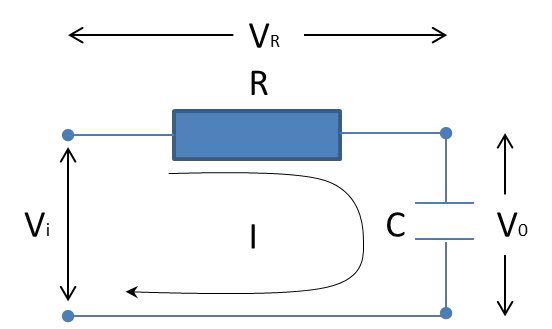
\includegraphics[width=9cm]{rc.pdf}
\caption{Circuito RC}
\label{fig:RC}
\end{figure}

La intensidad eléctrica que atraviesa un condensador depende de su capacidad, y de la variación con respecto al tiempo del voltaje entre sus extremos,

\begin{equation*}
I=c\frac{dV_o}{dt}
\end{equation*}

La intensidad que atraviesa la resistencia se puede obtener a partir de la ley de Ohm,

\begin{equation*}
V_R=I\cdot R
\end{equation*}

Por otro lado, la intensidad que recorre el circuito es común para la resistencia y el condensador. El voltaje suministrado tiene que ser la suma de las caídas de voltaje en la resistencia y en el condensador, $V_i=V_o+V_R$. Sustituyendo y despejando,

\begin{equation*}
V_i=V_o+V_R \rightarrow V_i=V_o+I\cdot R \rightarrow V_i=V_o+R\cdot C\frac{dV_0}{dt}
\end{equation*}

Si reordenamos el resultado, 

\begin{equation*}
\frac{dV_o}{dt}=\frac{V_i-V_o}{R \cdot C}
\end{equation*}

Obtenemos una ecuación diferencial para el valor del voltaje en los extremos del condensador que puede tratarse como un  problema de valor inicial. Para este problema, la función $f(t,x)$ toma la forma,

\begin{equation*}
f(t,x) \equiv \frac{V_i-V_o}{R \cdot C}
\end{equation*}

además necesitamos conocer un valor inicial $V_o(0)$ para el voltaje en el condensador. Si suponemos que el condensador se encuentra inicialmente descargado, entonces $V_o(0)=0$. Para este problema se conoce la solución analítica. El voltaje del condensador en función del tiempo viene dado por la función,

\begin{equation*}
V_0(t)=V_i\left(1-e^{-t/R\cdot C}\right)
\end{equation*} 


Podemos resolver el problema de la carga del condensador, empleando el código de la función de Euler incluido más arriba. Lo único que necesitamos es definir una función de Matlab  para representar la función $f(x,t)$ de nuestro problema de valor inicial,
t
\begin{verbatim}
function s=condensador(~,Vo)
%t tiempo en este ejemplo la función no depende del tiempo por lo que esta
%variable realmente no se usa... pero como el programa Euler se la pasa, 
%empleamos el simbolo ~ para que no de errores...
%Vo Valor del voltaje en cada iteración

%hay que definir los parametros fijos del circuito...
C=0.0001; %Capacidad del condesador en Faradios
R=1000; %resitencia en Ohmios
%el voltaje de entrada podría Vi podria ser una función del tiempo... Aquí
%vamos a considerar que es constante...
Vi=10; %Voltaje suministrado al circuito en Voltios
%Aqui cosntruimos la funcion que representa el circuito RC,

s=(Vi-Vo)/R/C;
\end{verbatim}

\begin{figure}[h]
\centering
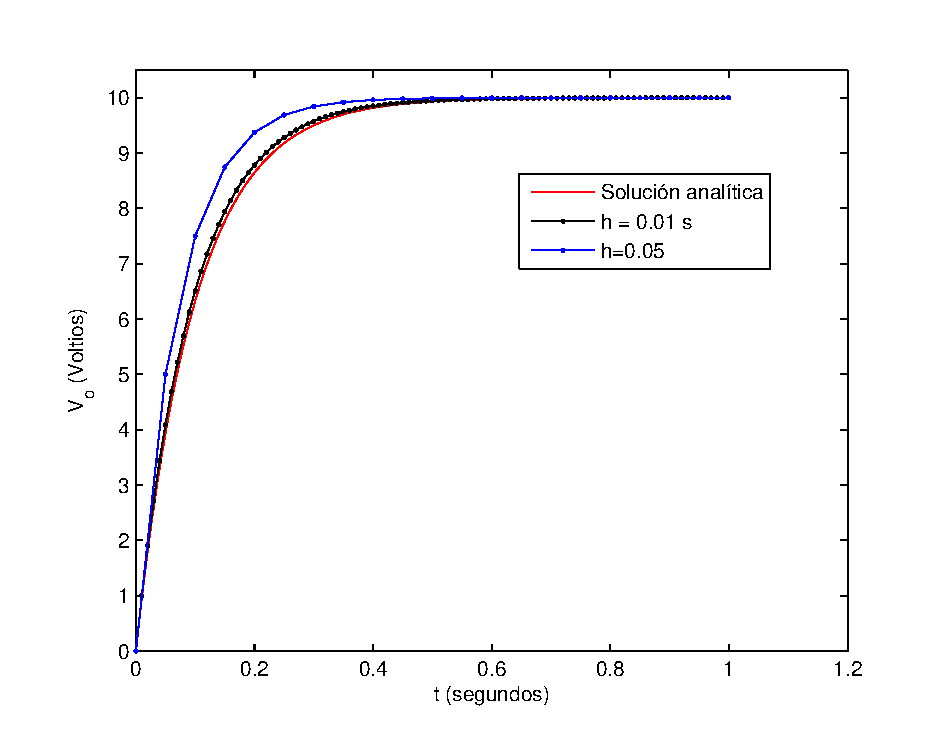
\includegraphics[width=12cm]{solrc.eps}
\caption{Comparacion entre los resultados obtenidos mediante el método de Euler para dos pasos de integración $h=0.05$ y $h=0.001$ y la solución analítica para el voltaje $V_o$ de un condensador durante su carga.}
\label{fig:solrc}
\end{figure}

La figura \ref{fig:solrc} compara gráficamente los resultados obtenido si empleamos la función descrita más arriba, \texttt{euler('condensador',0,0,1,h)}, para obtener el resultado de aplicar al circuito un voltaje de entrada constante $V_i=10$V durante un segundo, empleando dos pasos de integración distintos $h=0.05$s  y $h=0.01$s. Además, se ha añadido a la gráfica el resultado analítico.

En primer lugar, es interesante observar como el voltaje $V_0$ crece hasta alcanzar el valor $V_i=10$ V del voltaje suministrado al circuito. El tiempo que tarda el condensador en alcanzar dicho voltaje y quedar completamente cargado depende de su capacidad y de la resistencia presente en el circuito.

Como era de esperar, al hacer menor el paso de integración la solución numérica se aproxima más a la solución analítica. Sin embargo, como pasaba en el caso de los métodos de diferenciación de funciones, hay un valor de $h$ óptimo. Si disminuimos el paso de integración por debajo de ese valor, los errores de redondeo empiezan a dominar haciendo que la solución empeore.

\subsection{Métodos de Runge-Kutta} \index{Método de Runge-Kutta}
Si intentamos emplear polinomios de Taylor de grado superior, al empleado en el método de Euler, nos encontramos con la dificultad de obtener las derivadas sucesivas, con respecto al tiempo, de la función $f$. Así, si quisiéramos emplear el polinomio de Taylor de segundo grado, para la función x, tendríamos,
\begin{equation*}
x(t_{i+1})=x(t_i)+h\cdot f(t_i,x_i)+\frac{h^2}{2}f'(t_i,y_i)
\end{equation*}
Pero,
\begin{equation*}
f'(t,x)=\frac{\partial f(t,x)}{\partial t}+\frac{\partial f(t,x)}{\partial x}\cdot f(t,x)
\end{equation*}
Sacando factor común a h, obtenemos,
\begin{equation*}
x(t_{i+1})=x(t_i)+h\left(f(t_i,x_i)+\frac{h}{2}\left(\frac{\partial f(t_i,x_i)}{\partial t}+\frac{\partial f(t_i,x_i)}{\partial x}\cdot f(t_i,x_i)\right)\right)
\end{equation*}

A partir de este resultado, es fácil comprender que resulte complicado obtener métodos de resolución basados en el desarrollo de Taylor. De hecho, se vuelven cada vez más complicados según vamos empleando polinomios de Taylor de mayor grado.

Desde un punto de vista práctico, lo que se hace es buscar aproximaciones a los términos sucesivos del desarrollo de Taylor, para evitar tener que calcularlos explícitamente. Estas aproximaciones se basan a su vez, en el desarrollo de Taylor para funciones de dos variables.

Los métodos de integración resultantes, se conocen con el nombre genérico de métodos de Runge-Kutta. Veamos cómo se haría para el caso que acabamos de mostrar del polinomio de Taylor de segundo grado.

En primer lugar obtenemos el desarrollo del polinomio de Taylor de primer grado, en dos variables de la función $f(t,x)$, en un entorno del punto $t_i,x_i$,
\begin{equation*}
f(t,x)=f(t_i,x_i)+\left((t-t_i)\frac{\partial f(t_i,x_i)}{\partial t}+(x-x_i)\frac{\partial f(t_i,x_i)}{\partial x}\right)
\end{equation*}

Si ahora comparamos este resultado con la ecuación anterior, podríamos tratar de identificar entre sí los términos que acompañan las derivadas parciales, 

\begin{align*}
t-t_i&=\frac{h}{2} \rightarrow t=t_i+\frac{h}{2}\\
x-x_i&=\frac{h}{2}\cdot f(t_i,x_i) \rightarrow x=x_i+\frac{h}{2}\cdot f(t_i,x_i)
\end{align*}

Es decir,

\begin{equation*}
f(t_i,x_i)+\frac{h}{2}\left(\frac{\partial f(t_i,x_i)}{\partial t}+\frac{\partial f(t_i,x_i)}{\partial x}\cdot f(t_i,x_i)\right)=f(t_i+\frac{h}{2},x_i+\frac{h}{2}\cdot f(t_i,x_i))
\end{equation*}

Si ahora sustituimos este resultado en nuestra expresión del polinomio de Taylor de segundo grado de la función $x(t)$,

\begin{equation*}
x(t_{i+1})=x(t_i)+h\cdot f(t_i+\frac{h}{2},x_i+\frac{h}{2}f(t_i,x_i))
\end{equation*}
Donde $x_i\equiv x(t_i)$. Esta aproximación da lugar al primero y más sencillo de los métodos de Runge-Kutta, conocido como método del punto medio. El nombre es debido a que la función $f$ se evalúa en un punto a mitad de camino entre $t_i$ y $t_{i+1}=t_i+h$. El cálculo de la solución de un problema de valor inicial mediante este método, se puede expresar de un modo análogo al del método de Euler, 
\begin{align*}
x_0&=x(a)\\
x_1&=x_0+h\cdot f(a+\frac{h}{2},x_0+\frac{h}{2}f(a,x_0))\\
\vdots \\
x_{i+1}&=x_i+h\cdot f(t_i+\frac{h}{2},x_i+\frac{h}{2}f(t_i,x_i))\\
\end{align*}
La siguiente función de Matlab implementa el método del punto medio,

\begin{verbatim}
function y=pmedio(fun,ya,a,b,h)
%metodo de rungekutta de segundo orden mas conocido como del punto medio
%uso: y=pmedio(fun,ya,a,b,h)
% variables de entrada: fun, nombre entre comillas de la función que define
% el problema de valor inicial que se desea resolver. ya, valor inicial. a,
% instante de tiempo inicial o valor inicial de la variable independiente.
% b valor de tiempo final o valor final de la variable independiente. h,
% paso de integracion
%podemos por elemental prudencia, comprobar que b>a
%lo elegante no es pasar el paso como he hecho aqui, sino calcularlo en
%funcion de cuantos puntos de la solucion queremos en el intervalo...
if a>=b
    y='el intervalo debe ser creciente, para evitarse lios'
    return
end
y=ya;
paso=1;
t(paso)=a;
while t(paso)<=b
    t(paso+1)=t(paso)+h;
    y(paso+1)=y(paso)+h*feval(fun,t(paso)+h/2,y(paso)+h*feval(fun,t(paso),y(paso))/2);
    paso=paso+1;
end
%pintamos la solucion,
plot(t,y)

\end{verbatim}


El resto de los métodos de Runge-Kutta, los dejaremos para cuando seáis más mayores... Pero que conste que es de lo más interesante de los métodos numéricos.